% Provenance (never printed): old terminale S material on the disappearance of
% mountain ranges (erosion, transport, sedimentation, isostatic rebound, the
% recycling of continental material). Owner (Sync 0/1): denudation rate,
% sediment load (bed, suspended, dissolved), isostatic rebound, detrital rock,
% diagenesis. Weathering, erosion, deposition are Book 1's (g5); hydrolysis and
% clay minerals g10.07's; discharge g10.08's; isostasy and Airy's model g11.03's;
% sedimentary basin g11.09's; mountain root g12.01's; metamorphism g12.03's;
% half-life is physics' (recalled in prose). Figures: figdata/grade-12/relief_decay.py
% (rates, decay curves, the Varden unconformity from figdata/shared/region.py).
\chapter{La destrucción de las montañas}\label{ch:g12:destruction-of-mountains}

Vistos desde la Estación Espacial Internacional, los montes Apalaches del este
de América del Norte forman un llamativo dibujo de largas crestas oscuras y
boscosas y de valles claros y cultivados, más de \qty{500}{km} de ellos en la
fotografía de abajo. Las crestas son capas de roca dura que se arrugaron en
\omterm{def:g12:mountain-building:fold}{pliegues} apretados cuando África empujó contra América del Norte, en los
periodos Carbonífero y Pérmico, hace más de 250 millones de años. Hoy su
cumbre más alta, el monte Mitchell, el punto más alto al este del río
Misisipi, se eleva \qty{2037}{m} sobre el nivel del mar, menos de la cuarta
parte de la altura del Everest.
% ledger: photo:g12-appalachians, usgs:alleghanian, usgs:alleghanian-age, ics:base.Triassic, ncparks:mitchell (6684 ft), tht:everest (Book 1 row, 8848.86 m)

\begin{omfigure}
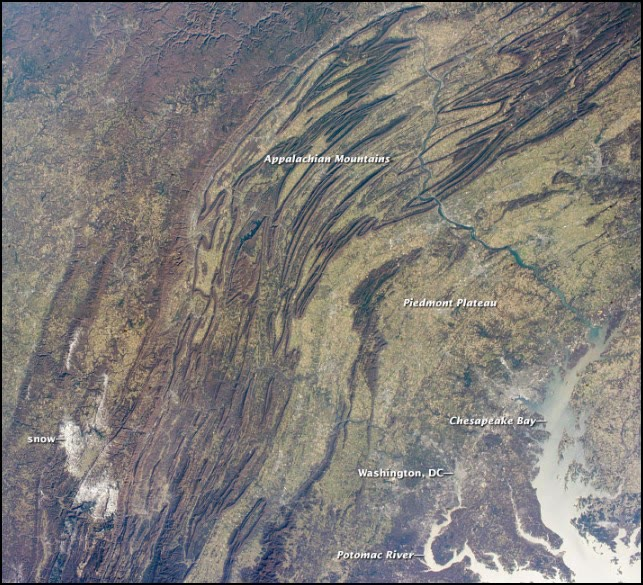
\includegraphics[width=0.6\linewidth]{images/book2/g12-iss-appalachians.jpg}

{\small Los Apalaches de valles y crestas, del noreste de Pensilvania (arriba
a la derecha) a Virginia Occidental, fotografiados desde la Estación Espacial
Internacional el 17 de noviembre de 2012. Las crestas boscosas son capas de
roca dura; los valles cultivados, capas más blandas. Fotografía de la NASA
(dominio público).}
\end{omfigure}
% ledger: photo:g12-appalachians

Una cordillera no dura. Desde el momento en que se eleva, la lluvia, el hielo
y los ríos la atacan; la roca que se llevan acaba en el mar, donde se
convierte en roca nueva. Este capítulo mide con qué rapidez ocurre eso, sigue
los derrubios hasta el lugar donde se convierten en piedra y muestra por qué
una cordillera que se desgasta sigue elevándose mientras tanto.

\begin{recall}
La meteorización descompone la roca allí donde está; la erosión se lleva los
derrubios y la sedimentación los deposita en otro lugar (Libro 1, año 5). La
\omterm{def:g10:soil-formation:chemical-weathering}{meteorización química} transforma los feldespatos en \omterm{def:g10:soil-formation:clay}{minerales de la arcilla}
por \omterm{def:g10:soil-formation:hydrolysis}{hidrólisis} (el \cref{ch:g10:soil-formation}). El \omterm{def:g10:drainage-basins:discharge}{caudal} de un río es el
volumen de agua que pasa por un punto en un segundo (el
\cref{ch:g10:drainage-basins}). La corteza flota sobre el manto en \omterm{def:g11:lithosphere-asthenosphere:isostasy}{isostasia};
en el modelo de Airy, una región cuya corteza es más gruesa en $\Delta H$ se
eleva $\Delta H\,(\rho_m - \rho_c)/\rho_m$ más
(el \cref{ch:g11:lithosphere-asthenosphere}), y una cordillera alta descansa
sobre una \omterm{def:g12:continental-crust:root}{raíz} de corteza gruesa (el \cref{ch:g12:continental-crust}). Los
sedimentos se acumulan en \omterm{def:g11:fossil-fuel-geology:basin}{cuencas sedimentarias} (el
\cref{ch:g11:fossil-fuel-geology}). Las rocas enterradas a gran profundidad en
un cinturón montañoso se metamorfizan (el \cref{ch:g12:metamorphic-rocks}).
\end{recall}

\section{¿Con qué rapidez se desgasta la tierra firme?}

\begin{definition}[Tasa de denudación]\label{def:g12:destruction-of-mountains:denudation}
La \emph{tasa de denudación}\index{tasa de denudacion@tasa de denudación} de una
región es el espesor medio de roca que la meteorización y la erosión juntas le
quitan por unidad de tiempo. Suele darse en metros por millón de años
(\unit{m/Myr}), lo mismo que milímetros por cada mil años.
\end{definition}
% ledger: pb11:rates (rates in m/Myr), earle:loads

¿Cómo puede medirse algo tan lento? Los rayos cósmicos que chocan con el
suelo producen un isótopo raro, el berilio 10, en el cuarzo de los primeros
metros de roca. Cuanto más despacio se desgasta una superficie, más tiempo
permanece cada grano cerca de ella, y más berilio 10 acumula. Medirlo en la
arena de un río da la \omterm{def:g12:destruction-of-mountains:denudation}{tasa de denudación} media de toda la cuenca situada aguas
arriba, a lo largo de los últimos miles a millones de años.
% ledger: pb11:rates (10Be produced within a few metres of the surface; concentration reflects near-surface residence time; 10^3 to 10^6 years)

Una recopilación de 1599 de estas medidas halló que los afloramientos de roca
desnuda se desgastan despacio, \qty{12}{m/Myr} de media (mediana de
\qty{5.4}{m/Myr}), y nunca más deprisa que \qty{140}{m/Myr}. Las \omterm{def:g10:drainage-basins:drainage-basin}{cuencas
hidrográficas} enteras pierden mucho más, \qty{218}{m/Myr} de media, pero con
una mediana de solo \qty{54}{m/Myr}: unas pocas cuencas rápidas tiran de la
media hacia arriba. Las más rápidas son las empinadas: la pendiente media de
una cuenca es el factor que mejor predice su tasa. Las cuencas de las regiones
sísmicamente activas, donde las montañas se están elevando, se erosionan
alrededor del doble de deprisa que las de regiones tranquilas.
% ledger: pb11:rates

\begin{omfigure}
\begin{tikzpicture}
\begin{axis}[omrecord, xbar, xmode=log, log origin=infty, bar width=7pt, bar shift=0pt,
  width=0.62\linewidth, height=6.6cm, scale only axis, xmin=3, xmax=1000,
  ymin=0.4, ymax=10.6, ytick={1,...,10}, y tick label style={font=\scriptsize, align=right},
  yticklabels={{afloramientos, mediana}, {afloramientos, media}, {ríos del mundo (balance)}, {cuencas, mediana},
    {Misisipi, antes de 1900 (balance)}, {cuencas áridas, media}, {cuencas tranquilas, media}, {cuencas, media},
    {cuencas sísmicamente activas, media}, {cuencas polares, media}},
  xlabel={tasa de denudación (\unit{m/Myr}), escala logarítmica}, ymajorgrids=false,
  unbounded coords=discard, nodes near coords, nodes near coords align={horizontal}, nodes near coords style={font=\scriptsize},
  point meta=rawx, every node near coord/.append style={/pgf/number format/.cd, fixed, precision=0}]
% computed in figdata/grade-12/relief_decay.py; ledger: pb11:rates, mm10:mississippi, kammerer:mississippi, earle:loads, cm95:crust
\addplot[fill=omThm!45, draw=omThm, every node near coord/.append style={/pgf/number format/.cd, fixed, precision=1}] table[x=measured, y=idx] {figdata/out/grade-12-relief_decay-rates.dat};
\addplot[fill=omDef!45, draw=omDef] table[x=budget, y=idx] {figdata/out/grade-12-relief_decay-rates.dat};
\end{axis}
\end{tikzpicture}

{\small \omterm{def:g12:destruction-of-mountains:denudation}{Tasas de denudación} medidas con berilio 10 (en rojo: 1599 medidas,
1149 de ellas en arena de río) y dos tasas calculadas en este capítulo a
partir del sedimento que transportan los ríos (en azul). Fuentes: Portenga y
Bierman (2011); Meade y Moody (2010); Syvitski y otros (2005).}
\end{omfigure}
% values: world_m_per_myr 43.5, miss_before_1900_m_per_myr 55.8 (relief_decay.py)

\section{Los ríos se llevan las montañas}

Gran parte de lo que se desgasta de la tierra firme sale de ella por los ríos.

\begin{definition}[Carga sedimentaria]\label{def:g12:destruction-of-mountains:load}
La \emph{carga sedimentaria}\index{carga sedimentaria} de un río es el
material que transporta, en tres formas: la \emph{carga de
fondo}\index{carga de fondo}, granos grandes que ruedan, son empujados o saltan
por el lecho; la \emph{carga en suspensión}\index{carga en suspension@carga en suspensión},
granos pequeños sostenidos en el agua en movimiento; y la \emph{carga
disuelta}\index{carga disuelta}, iones en disolución, como el calcio y el
cloruro, que deja la \omterm{def:g10:soil-formation:chemical-weathering}{meteorización química}.
\end{definition}
% ledger: earle:loads

Por término medio, la \omterm{def:g12:destruction-of-mountains:load}{carga disuelta} es alrededor del \qty{15}{\percent} de la
masa que transporta un río. Cuanto más rápida es el agua, mayores son los
granos que puede levantar. Un grano de arena de \qty{1}{mm} se levanta del
lecho a unos \qty{20}{cm/s} y, una vez en movimiento, permanece en suspensión
hasta que la corriente baja de \qty{10}{cm/s}. Los granos de limo son más
difíciles de levantar que la arena, porque se pegan entre sí: un grano de
\qty{0.01}{mm} necesita \qty{60}{cm/s} para levantarse, pero después una
corriente de \qty{0.1}{cm/s} lo mantiene en suspensión. Por eso los ríos en
crecida bajan pardos, y por eso el fango más fino viaja hasta el mar.
% ledger: earle:loads

\begin{omfigure}
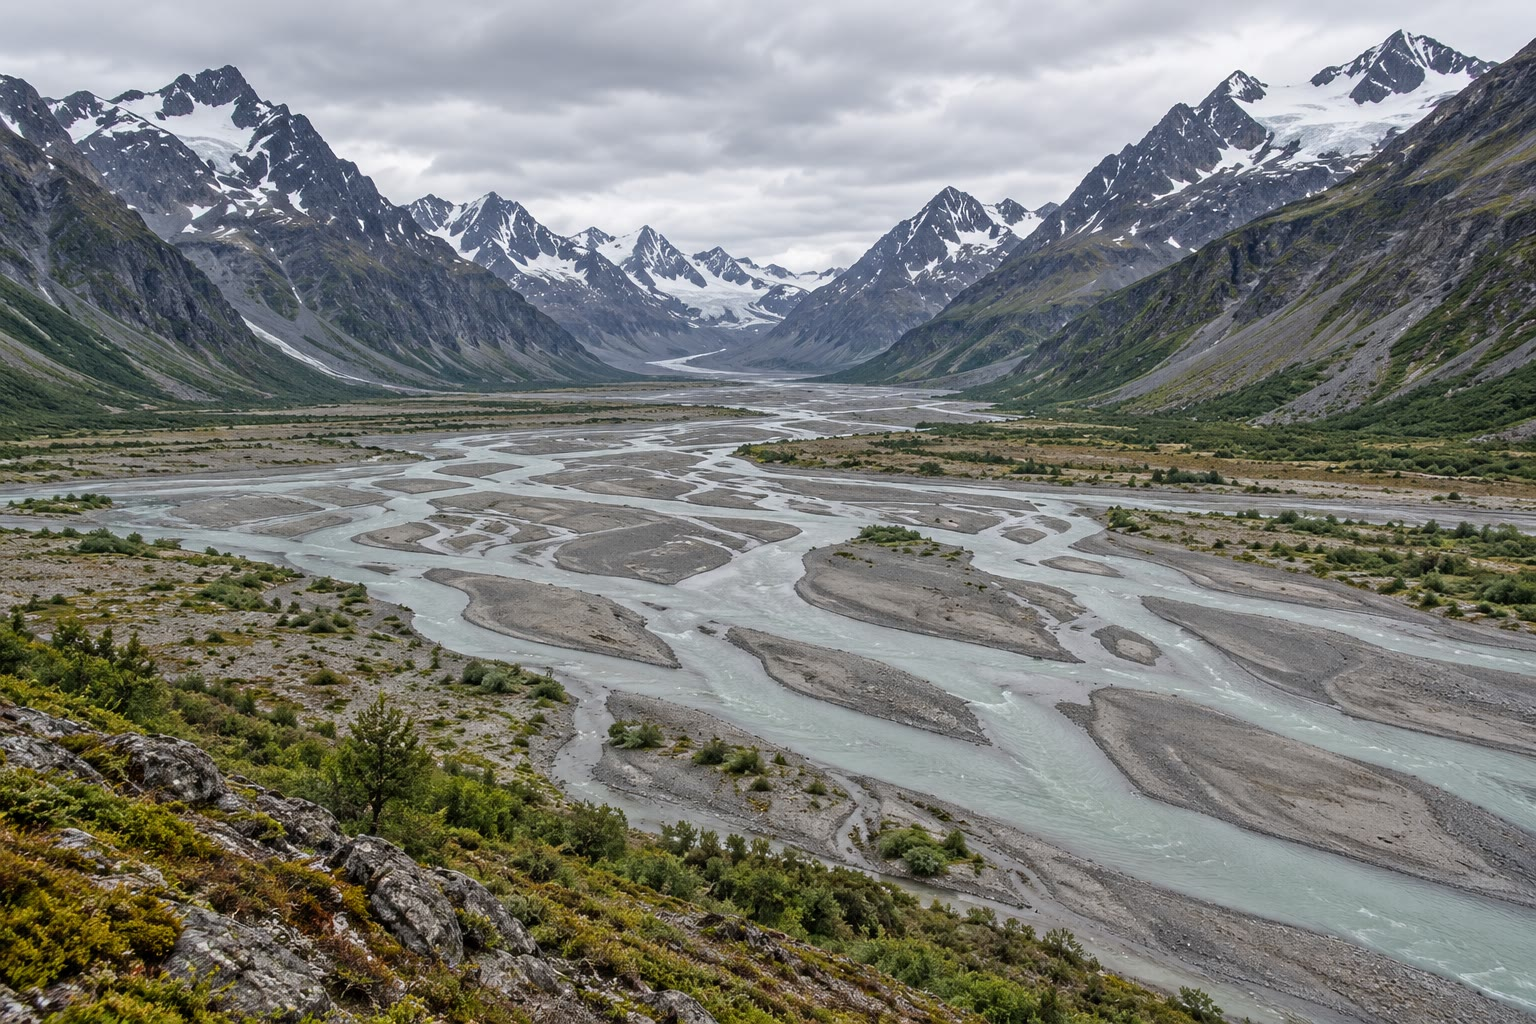
\includegraphics[width=0.66\linewidth]{images/book2/ai/g12-braided-river.jpg}

{\small Un río trenzado en un valle de montaña glaciar: canales poco profundos
que se separan y se vuelven a unir entre barras de grava que el agua solo
mueve en las crecidas. Ilustración generada por IA.}
\end{omfigure}

Medir lo que transporta un río da una segunda forma de hallar una \omterm{def:g12:destruction-of-mountains:denudation}{tasa de denudación}.

\begin{method}[Un balance de erosión]\label{met:g12:destruction-of-mountains:budget}
\begin{enumerate}
  \item Toma la masa de sedimento que transporta el río en un año y súmale la
        \omterm{def:g12:destruction-of-mountains:load}{carga disuelta} (si solo se conoce la carga sólida, divídela por
        $0.85$).
  \item Divide por la densidad de la roca, unos \qty{2830}{kg/m^3} para la
        \omterm{def:g12:continental-crust:continental-crust}{corteza continental}, para obtener el volumen de roca quitado cada año.
  \item Divide por la superficie de la \omterm{def:g10:drainage-basins:drainage-basin}{cuenca hidrográfica}: es el espesor
        quitado cada año.
  \item Multiplica por $10^6$ para expresarlo en metros por millón de años.
\end{enumerate}
\end{method}
% ledger: earle:loads, cm95:crust

\begin{example}[El Misisipi]\label{ex:g12:destruction-of-mountains:mississippi}
Antes de 1900, el sistema fluvial Misuri--Misisipi llevaba al mar unos 400
millones de toneladas de sedimento al año, desde una cuenca de unos
\qty{2980000}{km^2}. Con la \omterm{def:g12:destruction-of-mountains:load}{carga disuelta}, $400/0.85 \approx 471$ millones de
toneladas, es decir, $\num{4.71e11}/2830 \approx \qty{1.66e8}{m^3}$ de roca al
año. Repartido sobre $\qty{2.98e12}{m^2}$, forma una capa de
\[
  \frac{\num{1.66e8}}{\num{2.98e12}} \approx \qty{5.6e-5}{m}
  \text{ al año, unos } \qty{56}{m/Myr}.
\]
Entre 1987 y 2006, el río solo llevó 145 millones de toneladas al año, lo que
da unos \qty{20}{m/Myr}: las presas construidas en el Misuri en la década de
1950 retienen de 100 a 150 millones de toneladas al año, y otras obras
retienen más.
\end{example}
% ledger: mm10:mississippi, kammerer:mississippi, earle:loads, cm95:crust
% values: miss_before_1900_m_per_myr 55.8, miss_1987_2006_m_per_myr 20.2 (relief_decay.py)

Se puede hacer el mismo balance para el mundo entero. Antes de que el ser
humano modificara los ríos, estos llevaban a las costas unos 15\,500 millones
de toneladas de sedimento sólido al año; con la \omterm{def:g12:destruction-of-mountains:load}{carga disuelta}, son unos
\qty{6.4}{km^3} de roca al año, quitados de los \qty{1.48e8}{km^2} de los
continentes: una \omterm{def:g12:destruction-of-mountains:denudation}{tasa de denudación} media de unos \qty{43}{m/Myr}, cercana a
la mediana de las medidas de berilio 10. Desde entonces, el ser humano ha
cambiado los dos términos: la erosión del suelo ha aumentado lo que recogen
los ríos en unos 2300 millones de toneladas al año, pero más de 100\,000
millones de toneladas de sedimento están hoy retenidas tras las presas.
% ledger: syvitski:modern-flux (Book 1 row, prehuman 15.5 Gt/yr with bed load), sy05:humans, data:etopo1 (land fraction 0.290, grade-11 hypsometry), cm95:crust
% values: world_volume_km3_per_yr 6.44, land_area_km2 1.48e8, world_m_per_myr 43.5 (relief_decay.py)

\section{Del sedimento a la roca}

Lo que transportan los ríos se deposita donde la corriente se frena: en
valles y lagos, en deltas y, sobre todo, en las \omterm{def:g11:fossil-fuel-geology:basin}{cuencas sedimentarias} de los
márgenes continentales. Capa tras capa, el sedimento queda enterrado y se
convierte lentamente en roca.

\begin{definition}[Roca detrítica; diagénesis]\label{def:g12:destruction-of-mountains:diagenesis}
Una \emph{roca detrítica}\index{roca detritica@roca detrítica} (o roca clástica) es una
roca sedimentaria formada por fragmentos, los clastos, de rocas y minerales
más antiguos. La \emph{diagénesis}\index{diagenesis@diagénesis} es el conjunto de
cambios que convierten un sedimento enterrado en roca a baja temperatura: la
\emph{compactación}, cuando el peso de las capas de encima expulsa el agua y
el aire, y después la \emph{cementación}, cuando los minerales que cristalizan
a partir del agua de los poros (calcita, cuarzo, hematites, \omterm{def:g10:soil-formation:clay}{minerales de la
arcilla}) pegan los granos entre sí.
\end{definition}
% ledger: earle:clastic

Las \omterm{def:g12:destruction-of-mountains:diagenesis}{rocas detríticas} se nombran según el tamaño de sus clastos:
\begin{itemize}
  \item un \textbf{conglomerado} está formado por clastos redondeados de más
        de \qty{2}{mm}, y una \textbf{brecha}, por clastos angulosos;
  \item una \textbf{arenisca} está formada por arena, granos de entre
        \qty{2}{mm} y \qty{0.063}{mm}, casi siempre de cuarzo, el mineral que
        mejor resiste la meteorización;
  \item una \textbf{roca lutítica} contiene al menos un \qty{75}{\percent} de
        limo y arcilla; es una lutita si se separa en capas finas.
\end{itemize}
% ledger: earle:clastic

\begin{omfigure}
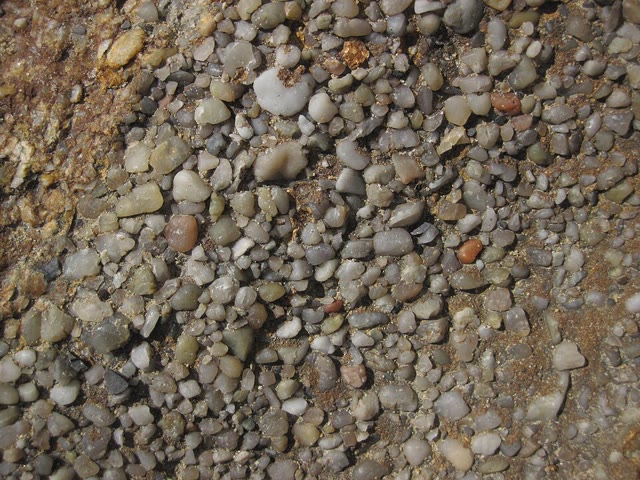
\includegraphics[width=0.5\linewidth]{images/book2/g12-stjohn-conglomerate.jpg}

{\small Un conglomerado de cantos de cuarzo de Ohio, de edad carbonífera:
cantos redondeados de cuarzo cementados por arena más fina. Fotografía de
James St.~John (CC~BY~2.0).}
\end{omfigure}
% ledger: photo:g12-conglomerate, ics:base.Carboniferous, ics:base.Permian (Lower Pennsylvanian lies in the Carboniferous)

Los clastos registran el viaje. Los cantos redondeados han rodado mucho en un
río o en una playa; los angulosos apenas han viajado. Una arenisca formada
casi solo por cuarzo procede de una roca que estuvo meteorizándose mucho
tiempo, hasta que los demás minerales se convirtieron en arcilla.
% ledger: earle:clastic (rounded/angular, most sand grains quartz, the most resistant mineral)

\section{La raíz asciende}

Si la erosión se limitara a quitar roca de la parte alta de una cordillera,
una cordillera de \qty{2}{km} de altura, desgastada a \qty{200}{m/Myr},
desaparecería en diez millones de años. Pero la cordillera flota sobre el
manto. A medida que se quita roca de arriba, la columna se aligera, y sube.

\begin{definition}[Rebote isostático]\label{def:g12:destruction-of-mountains:rebound}
El \emph{rebote isostático}\index{rebote isostatico@rebote isostático} es la
elevación de una región de la \omterm{def:g11:lithosphere-asthenosphere:lithosphere}{litosfera} cuando se le quita una carga ---roca
desgastada por la erosión, o un casquete de hielo que se funde--- hasta que se
restablece la \omterm{def:g11:lithosphere-asthenosphere:isostasy}{isostasia}.
\end{definition}
% ledger: sella07:gia (rebound after ice unloading)

\begin{proposition}[Erosión y rebote]\label{prop:g12:destruction-of-mountains:rebound}
En el modelo de Airy, cuando la erosión quita un espesor $e$ de corteza de
densidad $\rho_c$ a una región en \omterm{def:g11:lithosphere-asthenosphere:isostasy}{isostasia} sobre un manto de densidad
$\rho_m$, la superficie solo baja
\[
  \Delta h = e\left(1 - \frac{\rho_c}{\rho_m}\right),
\]
mientras que la base de la corteza sube $e\,\rho_c/\rho_m$.
\end{proposition}

\begin{proof}
Quitar $e$ de arriba hace la corteza más delgada en $e$. Según el modelo de
Airy, una corteza más delgada en $e$ queda más baja en $e\,(\rho_m - \rho_c)/\rho_m = e(1 -
\rho_c/\rho_m)$. La parte superior de la corteza ha bajado esa cantidad, y su
espesor ha disminuido en $e$, así que su base ha subido $e - e(1 -
\rho_c/\rho_m) = e\,\rho_c/\rho_m$.
\end{proof}

Con $\rho_c = \qty{2830}{kg/m^3}$ y $\rho_m = \qty{3380}{kg/m^3}$, $1 -
\rho_c/\rho_m \approx 0.163$. Quitar \qty{1}{km} de roca solo baja la
superficie unos \qty{163}{m}: los otros \qty{837}{m} los compensa la subida de
toda la columna. Para bajar una cordillera \qty{2000}{m}, la erosión debe
quitar unos $2000/0.163 \approx \qty{12300}{m}$ de roca. Rocas que estaban a
más de \qty{12}{km} de profundidad, rocas metamórficas y granitos formados en
las profundidades de la cordillera, llegan a la superficie: por eso los
antiguos cinturones montañosos desgastados dejan al descubierto esquistos,
gneises y granitos en extensiones enormes.
% ledger: cm95:crust, data:prem (rho 3.38 below the Moho)
% values: rebound_fraction 0.16272, lowering_per_km_m 162.7, root_rise_per_km_m 837.3, eroded_for_2000m_km 12.29 (relief_decay.py)

\begin{omfigure}
\begin{tikzpicture}[x=1cm, y=1cm, font=\scriptsize]
  % three columns: before, after erosion without rebound, after rebound
  \foreach \i/\top/\base/\lab in {0/3.0/-3.2/{una cordillera en isostasia}, 1/2.0/-3.2/{la erosión quita $e$}, 2/2.84/-2.36/{la columna sube}} {
    \begin{scope}[xshift=\i*4.6cm]
      \fill[omLithPeridotite!45] (0,-3.6) rectangle (3.4,-0.6);
      \fill[omLithGranite!55, draw=black!60] (0.5,\base) -- (0.5,0) -- (1.0,\top) -- (2.4,\top) -- (2.9,0) -- (2.9,\base) -- cycle;
      \fill[omLithGranite!55, draw=black!60] (0,0) rectangle (0.5,-0.6);
      \fill[omLithGranite!55, draw=black!60] (2.9,0) rectangle (3.4,-0.6);
      \draw[black!40, densely dashed] (-0.1,0) -- (3.5,0);
      \node[anchor=north, align=center, text width=3.4cm] at (1.7,-3.75) {\lab};
    \end{scope}
  }
  % eroded slab, middle panel
  \draw[omThm, densely dashed] (4.6+1.0,3.0) -- (4.6+2.4,3.0);
  \draw[omThm, |-|] (4.6+2.65,3.0) -- node[right] {$e$} (4.6+2.65,2.0);
  % right panel: the old top and base
  \draw[omThm, densely dashed] (9.2+1.0,3.0) -- (9.2+2.4,3.0);
  \draw[omThm, densely dashed] (9.2+0.5,-3.2) -- (9.2+2.9,-3.2);
  \draw[-{Stealth}, omDef, line width=0.9pt] (9.2+1.7,-3.15) -- (9.2+1.7,-2.45);
  \node[omDef, anchor=west] at (9.2+3.0,-2.8) {la raíz sube};
  \node[anchor=west] at (9.2+3.0,2.95) {superficie más baja};
  \node[anchor=west] at (9.2+3.0,2.55) {solo en $0.16\,e$};
  \draw[black!60, |-|] (9.2+2.65,3.0) -- (9.2+2.65,2.84);
  % labels
  \node[anchor=west] at (3.45,-2.1) {manto};
  \node at (1.7,-1.5) {corteza};
\end{tikzpicture}

{\small Erosión y \omterm{def:g12:destruction-of-mountains:rebound}{rebote isostático} (esquema, alturas sin escala). A la
izquierda: una cordillera en \omterm{def:g11:lithosphere-asthenosphere:isostasy}{isostasia}, con su \omterm{def:g12:continental-crust:root}{raíz}. En el centro: la erosión
quita un espesor $e$ de la parte alta. A la derecha: la columna, más ligera,
sube hasta que se restablece la \omterm{def:g11:lithosphere-asthenosphere:isostasy}{isostasia}; la superficie acaba solo
$0.163\,e$ más baja que al principio, y la \omterm{def:g12:continental-crust:root}{raíz} ha subido $0.837\,e$.}
\end{omfigure}

El mismo rebote puede observarse hoy donde una carga desapareció deprisa. El
casquete de hielo que cubría gran parte de Canadá en el último máximo glacial
era más grueso en torno a la bahía de Hudson. Ese hielo se ha fundido, y el
terreno allí sigue elevándose: unos \qty{10}{mm} al año, según las medidas
GPS, es decir, \qty{10000}{m/Myr}, unas cincuenta veces la \omterm{def:g12:destruction-of-mountains:denudation}{tasa de
denudación} media de las \omterm{def:g10:drainage-basins:drainage-basin}{cuencas hidrográficas}. Más al sur, pasados los
Grandes Lagos, el terreno se hunde de 1 a \qty{2}{mm} al año.
% ledger: sella07:gia, pb11:rates

\section{¿Cuánto dura una cordillera?}

Cuanto más empinada es una cuenca, más deprisa se erosiona; en las cuencas
grandes, se ha hallado que la \omterm{def:g12:destruction-of-mountains:denudation}{tasa de denudación} es proporcional a su relieve
medio. Tomemos el modelo más sencillo que lo expresa.

\begin{proposition}[El decrecimiento exponencial de una cordillera]\label{prop:g12:destruction-of-mountains:decay}
Sea $h(t)$ la altitud media de una cordillera sobre las llanuras que la
rodean. Si la \omterm{def:g12:destruction-of-mountains:denudation}{tasa de denudación} es $E = k\,h$, con $k$ constante, y si la
\omterm{def:g11:lithosphere-asthenosphere:isostasy}{isostasia} se restablece en todo momento, entonces
\[
  h(t) = h_0\, e^{-f k t}, \qquad f = 1 - \frac{\rho_c}{\rho_m},
\]
donde $h_0$ es la altitud en $t = 0$. La altitud se divide por $e$ cada
$\tau = 1/(fk)$, y por dos cada $\tau \ln 2$.
\end{proposition}

\begin{proof}
En un tiempo corto $\mathrm{d}t$, la erosión quita un espesor $E\,\mathrm{d}t
= k h\,\mathrm{d}t$ y, por la proposición anterior, la superficie baja
$f k h\,\mathrm{d}t$. Así que $h' = -fk\,h$, y las soluciones de esta
ecuación son $h(t) = h_0\,e^{-fkt}$. En $t = \tau$, $h = h_0/e$; $h = h_0/2$
cuando $fkt = \ln 2$.
\end{proof}

Las medidas en grandes cuencas dan $k$: sin ningún levantamiento, su relieve
caería a la décima parte en unos 11 millones de años. Así que $e^{-11k} = 0.1$, y $k =
\ln 10/11 \approx 0.209$ por millón de años. Sin rebote ($f = 1$), la
constante de tiempo sería $1/k \approx 4.8$ millones de años. Con rebote, $f
\approx 0.163$ y
\[
  \tau = \frac{1}{0.163 \times 0.209} \approx 29 \text{ millones de años},
\]
y la altitud media se reduce a la mitad cada $29 \ln 2 \approx 20$ millones de
años: el rebote hace que una cordillera dure unas seis veces más.
% ledger: ahnert70:decay, cm95:crust, data:prem
% values: k_per_myr 0.20933, tau_none_myr 4.777, tau_rebound_myr 29.36, half_rebound_myr 20.35, half_none_myr 3.31 (relief_decay.py)

\begin{omfigure}
\begin{tikzpicture}
\begin{axis}[omrecord, width=0.7\linewidth, height=5.4cm, xmin=0, xmax=100, ymin=0, ymax=2100,
  xlabel={tiempo (millones de años)}, ylabel={altitud media (\unit{m})},
  xtick={0,20,...,100}, ytick={0,500,...,2000}]
% computed in figdata/grade-12/relief_decay.py; ledger: ahnert70:decay, cm95:crust, data:prem
\addplot[omProp, line width=1.1pt, densely dashed] table[x=t_Myr, y=h_none] {figdata/out/grade-12-relief_decay-curve.dat};
\addplot[omDef, line width=1.1pt] table[x=t_Myr, y=h_rebound] {figdata/out/grade-12-relief_decay-curve.dat};
\draw[black!45, densely dotted] (axis cs:20.35,0) -- (axis cs:20.35,1000) -- (axis cs:0,1000);
\draw[omProp, line width=0.4pt] (axis cs:9,304) -- (axis cs:33,215);
\coordinate (none) at (axis cs:33.5,215);
\coordinate (reb) at (axis cs:45,780);
\end{axis}
\node[font=\scriptsize, text=omProp, anchor=west] at (none) {sin rebote};
\node[font=\scriptsize, text=omDef, anchor=south west] at (reb) {con rebote};
\end{tikzpicture}

{\small La altitud media de una cordillera de \qty{2000}{m}, desgastada a un
ritmo proporcional a su altura, con y sin \omterm{def:g12:destruction-of-mountains:rebound}{rebote isostático}; con rebote,
queda la mitad de la altitud al cabo de 20 millones de años (punteado).
Constante de tasa de Ahnert (1970); densidades de la corteza y del manto bajo
el \omterm{def:g11:seismic-structure:moho}{Moho}.}
\end{omfigure}

Los Apalaches ponen a prueba esta imagen. Su colisión terminó en el Pérmico,
hace más de 250 millones de años. Eso es más de doce veces el tiempo que el
modelo tarda en reducir la altitud a la mitad: $2000 \times e^{-250/29} \approx
\qty{0.4}{m}$. Y, sin embargo, el monte Mitchell todavía se eleva
\qty{2037}{m} sobre el mar. El modelo por sí solo no puede explicar el relieve
actual: la región tiene que haberse elevado de nuevo desde entonces, o haberse
erosionado más despacio de lo que supone el modelo.
% ledger: usgs:alleghanian, usgs:alleghanian-age, ics:base.Triassic, ncparks:mitchell, ahnert70:decay
% values: h_after_250myr_rebound_m 0.40 (relief_decay.py)

Así, las montañas se reciclan. La roca desgastada de una cordillera acaba en
\omterm{def:g11:fossil-fuel-geology:basin}{cuencas sedimentarias}, donde se convierte en \omterm{def:g12:destruction-of-mountains:diagenesis}{roca detrítica}; una parte de esa
roca se entierra a la profundidad suficiente para metamorfizarse o incluso
fundirse, otra es arrastrada al manto en una \omterm{def:g11:subduction-zones:subduction}{zona de subducción} (el
\cref{ch:g12:subduction-magmatism}), y otra vuelve a plegarse en una nueva
cordillera cuando chocan dos continentes.
% ledger: ss09:balance (sediment subducted), earle:collision (sediments of both margins in the mountains)

\begin{omfigure}
\begin{tikzpicture}
\begin{axis}[omsection, x=1.25cm, y=0.003125cm, xmin=0, xmax=9.49, ymin=-700, ymax=650,
  xlabel={distancia desde A (\unit{km})}, ylabel={altitud (\unit{m})},
  ytick={-600,-300,0,300,600}, tick label style={font=\scriptsize}, unbounded coords=jump]
% shared region tables (figdata/shared/region.py); unconformity from figdata/grade-12/relief_decay.py; ledger: region:name
\addplot[fill=black!8, draw=black!50, line width=0.3pt, even odd rule] table {figdata/out/shared-region-section-unit-schist.dat};
\addplot[fill=icsTriassic!20, draw=black!50, line width=0.3pt, even odd rule] table {figdata/out/shared-region-section-unit-sandstone.dat};
\addplot[fill=icsJurassic!25, draw=black!50, line width=0.3pt, even odd rule] table {figdata/out/shared-region-section-unit-limestone.dat};
\addplot[fill=icsJurassic!8, draw=black!50, line width=0.3pt, even odd rule] table {figdata/out/shared-region-section-unit-shale.dat};
\addplot[fill=icsCretaceous!20, draw=black!50, line width=0.3pt, even odd rule] table {figdata/out/shared-region-section-unit-chalk.dat};
\addplot[fill=omLithAlluv, draw=black!50, line width=0.3pt, even odd rule] table {figdata/out/shared-region-section-unit-alluvium.dat};
\addplot[black, line width=0.7pt] table {figdata/out/shared-region-section-ground.dat};
\addplot[omThm, line width=1.4pt] table[x=s_km, y=z_m] {figdata/out/grade-12-relief_decay-unconformity.dat};
\addplot[fault] table {figdata/out/shared-region-section-fault.dat};
\node[anchor=south east, font=\small\bfseries] at (axis cs:0,650) {A};
\node[anchor=south west, font=\small\bfseries] at (axis cs:9.49,650) {B};
\node[font=\scriptsize, fill=white, inner sep=1pt] at (axis cs:1.2,-520) {esquisto, unos 480 Ma};
\coordinate (unc) at (axis cs:1.6,-300);
\end{axis}
\node[font=\scriptsize, text=omThm, anchor=west, fill=white, inner sep=1pt] at ([xshift=4pt]unc) {la discordancia};
\end{tikzpicture}

\smallskip
{\small\tikz\fill[black!8, draw=black!50] (0,0) rectangle (0.35,0.22);~esquisto \quad
\tikz\fill[icsTriassic!20, draw=black!50] (0,0) rectangle (0.35,0.22);~arenisca (Triásico) \quad
\tikz\fill[icsJurassic!25, draw=black!50] (0,0) rectangle (0.35,0.22);~caliza \quad
\tikz\fill[icsJurassic!8, draw=black!50] (0,0) rectangle (0.35,0.22);~lutita \quad
\tikz\fill[icsCretaceous!20, draw=black!50] (0,0) rectangle (0.35,0.22);~creta \quad
\omve{2.5}}

{\small Corte A--B a través de las Varden Hills, con la discordancia en rojo:
la base plana sobre la que se depositó la arenisca del Triásico encima del
zócalo de esquisto, plegada y fallada más tarde. Datos: el modelo de la región
de la serie.}
\end{omfigure}
% values: unconformity sampled from region.contact_elevation('sandstone'); varden_gap_myr 58.1 (relief_decay.py)

Las Varden Hills guardan el registro de un ciclo así. Su zócalo es un
esquisto, metamorfizado hace unos 480 millones de años, en el que se intruyó
un granito hace unos 310 millones de años ---los dos formados a kilómetros por
debajo de la superficie de un antiguo cinturón montañoso---. Sin embargo, la
arenisca del Triásico, depositada a partir de hace unos 252 millones de años,
descansa directamente sobre ellos, a través de una superficie plana: la
discordancia. En menos de 60 millones de años, aquella antigua cordillera se
había desgastado hasta formar una llanura, y sus rocas profundas habían
llegado a la superficie. Después, el mar se extendió sobre la llanura y la
enterró.
% ledger: region:name (model: schist 480 Ma, granite 310 Ma, erosion, unconformity, Triassic cover), ics:base.Triassic
% values: varden_gap_myr 58.1 (relief_decay.py)

\section{Ejercicios}

\begin{exercise}[$\star$]\label{exo:g12:destruction-of-mountains:1}
Da la palabra: (a) el espesor medio de roca quitado a una región por unidad de
tiempo; (b) los granos que un río hace rodar y saltar por su lecho; (c) los
iones que un río transporta en disolución; (d) los cambios que convierten un
sedimento enterrado en roca; (e) la elevación de la \omterm{def:g11:lithosphere-asthenosphere:lithosphere}{litosfera} cuando se le
quita una carga.
\end{exercise}

\begin{exercise}[$\star$]\label{exo:g12:destruction-of-mountains:2}
Nombra la \omterm{def:g12:destruction-of-mountains:diagenesis}{roca detrítica}: (1) cantos redondeados de \qtyrange{5}{20}{mm}
cementados entre sí; (2) granos de cuarzo de \qty{0.3}{mm}; (3) una roca con
un \qty{90}{\percent} de limo y arcilla que se separa en láminas finas;
(4) fragmentos angulosos de \qty{3}{cm}.
\end{exercise}

\begin{exercise}[$\star$]\label{exo:g12:destruction-of-mountains:3}
Convierte a milímetros al año: (1) \qty{54}{m/Myr}; (2) \qty{218}{m/Myr};
(3) y expresa en \unit{m/Myr} el levantamiento de \qty{10}{mm} al año cerca de la bahía de Hudson.
\end{exercise}

\begin{exercise}[$\star$]\label{exo:g12:destruction-of-mountains:4}
Un río transporta 60 millones de toneladas de sedimento sólido al año. Estima
su \omterm{def:g12:destruction-of-mountains:load}{carga disuelta}, sabiendo que la \omterm{def:g12:destruction-of-mountains:load}{carga disuelta} es, por término medio, el
\qty{15}{\percent} de la masa total transportada.
\end{exercise}

\begin{exercise}[$\star$]\label{exo:g12:destruction-of-mountains:5}
Ordena, desde la superficie hacia abajo, lo que le ocurre a un grano de cuarzo
de un granito: sedimentación en una cuenca, meteorización del granito,
enterramiento bajo capas más jóvenes, transporte por un río, cementación.
\end{exercise}

\begin{exercise}[$\star\star$]\label{exo:g12:destruction-of-mountains:6}
Una corriente se frena de \qty{30}{cm/s} a \qty{5}{cm/s}. Con los valores del
capítulo, di qué le ocurre a cada velocidad a un grano de arena de
\qty{1}{mm} que descansa en el lecho, y a un grano de limo de \qty{0.01}{mm}
que ya está en suspensión.
\end{exercise}

\begin{exercise}[$\star\star$]\label{exo:g12:destruction-of-mountains:7}
Una cuenca de \qty{50000}{km^2} envía al mar 4 millones de toneladas de
sedimento sólido al año. Haz su balance de erosión, incluida la \omterm{def:g12:destruction-of-mountains:load}{carga
disuelta}, con $\rho =
\qty{2830}{kg/m^3}$. Compáralo con la mediana de las
tasas de las cuencas medidas con berilio 10.
\end{exercise}

\begin{exercise}[$\star\star$]\label{exo:g12:destruction-of-mountains:8}
(1) Calcula $1 - \rho_c/\rho_m$ para $\rho_c = \qty{2700}{kg/m^3}$ y
$\rho_m = \qty{3300}{kg/m^3}$. (2) ¿Cuánto baja la superficie cuando se
erosiona \qty{1}{km} de roca? (3) Compáralo con el valor del capítulo.
\end{exercise}

\begin{exercise}[$\star\star$]\label{exo:g12:destruction-of-mountains:9}
Un granito cristalizó a unos \qty{8}{km} de profundidad bajo una cordillera.
(1) ¿Qué espesor de roca debe quitar la erosión para traerlo a la superficie?
(2) ¿Cuánto baja mientras tanto la superficie media? (3) A \qty{200}{m/Myr},
¿cuánto tiempo hace falta?
\end{exercise}

\begin{exercise}[$\star\star$]\label{exo:g12:destruction-of-mountains:10}
La altitud media de los continentes es de unos \qty{794}{m}. (1) A
\qty{43}{m/Myr}, ¿cuánto tardaría la erosión en quitar una capa de ese
espesor? (2) ¿Cuánto, si se tiene en cuenta el \omterm{def:g12:destruction-of-mountains:rebound}{rebote isostático} y la tasa no
cambia? (3) ¿Por qué, a pesar de todo, los continentes siguen elevándose sobre
el mar al cabo de 4000 millones de años?
\end{exercise}

\begin{exercise}[$\star\star$]\label{exo:g12:destruction-of-mountains:11}
Más de 100\,000 millones de toneladas de sedimento están retenidas tras
presas construidas en su mayoría en los últimos cincuenta años. (1) ¿Qué
volumen de roca es eso, a \qty{2830}{kg/m^3}? (2) ¿Cuántos años de la carga
sólida mundial anterior al ser humano, 15\,500 millones de toneladas al año,
representa?
\end{exercise}

\begin{exercise}[$\star\star\star$]\label{exo:g12:destruction-of-mountains:12}
Demuestra que, en el modelo del capítulo, la \omterm{def:g12:destruction-of-mountains:denudation}{tasa de denudación} de una
cordillera es $E(t) = k h_0 e^{-fkt}$. Calcula el espesor total de roca
quitado mientras la altitud media baja de $h_0$ a 0, y explica el resultado
con la proposición del rebote.
\end{exercise}

\begin{exercise}[$\star\star\star$]\label{exo:g12:destruction-of-mountains:13}
Cerca de la bahía de Hudson, el terreno se eleva \qty{10}{mm} al año. (1) Si
ese ritmo no cambiara, ¿cuánto se elevaría en 1000 años? (2) La elevación es
un rebote tras la fusión de un casquete de hielo. Toma un hielo de densidad
\qty{900}{kg/m^3} y el manto a \qty{3380}{kg/m^3}: ¿cuánto se elevaría el
terreno en total, en el modelo de Airy, tras la fusión de \qty{2}{km} de
hielo? (3) ¿Por qué debería frenarse el ritmo con el tiempo?
\end{exercise}
% ledger: sella07:gia, usgs:ice-density (ice about 90 % as dense as water), data:prem

\begin{exercise}[$\star\star\star$]\label{exo:g12:destruction-of-mountains:14}
El Misisipi transportaba 400 millones de toneladas de sedimento sólido al año
antes de 1900 y 145 millones de toneladas al año en 1987--2006. (1) Calcula la
\omterm{def:g12:destruction-of-mountains:denudation}{tasa de denudación} de su cuenca de \qty{2980000}{km^2} en los dos periodos,
con la \omterm{def:g12:destruction-of-mountains:load}{carga disuelta}. (2) ¿Cuál de las dos mide mejor la erosión natural de
la cuenca? (3) Las presas retienen de 100 a 150 millones de toneladas al año:
¿explica eso toda la disminución?
\end{exercise}

\begin{exercise}[$\star\star\star$]\label{exo:g12:destruction-of-mountains:15}
En las Varden Hills, un granito intruido hace unos 310 millones de años está
bajo la arenisca del Triásico, depositada a partir de hace unos 252 millones
de años. Supón que el granito cristalizó a \qty{6}{km} de profundidad. (1) ¿Qué
espesor de roca se quitó por encima de él, como mínimo? (2) ¿Qué \omterm{def:g12:destruction-of-mountains:denudation}{tasa de
denudación} media exige eso, como mínimo? (3) Compárala con las tasas medidas
en las cuencas.
\end{exercise}

\begin{problem}[{Problema de fin de semana --- ¿Cuánto se tarda en allanar una cordillera?}]
\label{pb:g12:destruction-of-mountains:1}
% ledger: pb11:rates, ahnert70:decay, cm95:crust, data:prem, usgs:alleghanian, usgs:alleghanian-age, ics:base.Triassic, ncparks:mitchell, photo:g12-appalachians
% values (relief_decay.py): k 0.20933/Myr, E0 418.7 m/Myr, f 0.16272, tau 4.777 / 29.36 Myr, half-lives 3.31 / 20.35 Myr
Una cordillera joven tiene una altitud media de \qty{2000}{m} sobre las
llanuras que la rodean. Sus ríos la desgastan a un ritmo proporcional a su
altura, $E = kh$, con $k = 0.209$ por millón de años. La corteza tiene una
densidad de \qty{2830}{kg/m^3}, y el manto de debajo, \qty{3380}{kg/m^3}.

\medskip
\noindent\textbf{Parte I --- La tasa de erosión.}
\begin{enumerate}
  \item Calcula la \omterm{def:g12:destruction-of-mountains:denudation}{tasa de denudación} actual de la cordillera, en \unit{m/Myr}.
  \item Exprésala en milímetros al año.
  \item Compárala con las tasas medias medidas en las cuencas sísmicamente
        activas (\qty{367}{m/Myr}) y en las tranquilas (\qty{182}{m/Myr}).
  \item ¿Qué característica de una cuenca predice mejor su tasa de erosión?
  \item ¿Cuántas toneladas de roca salen de cada kilómetro cuadrado de la
        cordillera cada año?
\end{enumerate}

\medskip
\noindent\textbf{Parte II --- Sin rebote.}
\begin{enumerate}[resume]
  \item Si la tasa se mantuviera en su valor actual, ¿cuánto se tardaría en
        quitar \qty{2000}{m} de roca?
  \item En realidad, la tasa baja a medida que la cordillera se rebaja.
        Escribe la ecuación $h' = -kh$ y su solución con $h(0) = \qty{2000}{m}$.
  \item ¿Cuál es la constante de tiempo $1/k$?
  \item ¿Cuánto tarda la altitud en reducirse a la mitad?
  \item Comprueba que al cabo de 11 millones de años queda la décima parte
        de la altitud.
\end{enumerate}

\medskip
\noindent\textbf{Parte III --- Con rebote.}
\begin{enumerate}[resume]
  \item Calcula $f = 1 - \rho_c/\rho_m$.
  \item Cuando se erosionan \qty{100}{m} de roca, ¿cuánto baja la superficie
        y cuánto sube la \omterm{def:g12:continental-crust:root}{raíz}?
  \item Escribe la nueva ecuación para $h$ y su solución.
  \item ¿Qué espesor de roca hay que erosionar para rebajar la cordillera de
        \qty{2000}{m} a \qty{200}{m}?
  \item ¿Qué tipos de roca trae eso a la superficie?
\end{enumerate}

\medskip
\noindent\textbf{Parte IV --- La constante de tiempo.}
\begin{enumerate}[resume]
  \item Calcula la constante de tiempo con rebote.
  \item ¿Cuánto tarda la cordillera en bajar a la décima parte de su altura?
  \item ¿Qué altura tiene al cabo de 200 millones de años?
  \item La colisión de los Apalaches terminó hace más de 250 millones de años.
        Si la cordillera nunca se hubiera vuelto a elevar, ¿qué altura le
        dejaría el modelo al cabo de 250 millones de años? El monte Mitchell
        todavía se eleva \qty{2037}{m} sobre el mar: ¿qué sugiere esto?
  \item En resumen: ¿en cuántos millones de años se reduce a la mitad la
        altitud media de la cordillera?
\end{enumerate}
\end{problem}
